\documentclass{standalone}
\usepackage{tikz}
\usetikzlibrary{patterns, positioning}
\usepackage[sfdefault]{ClearSans} %% option 'sfdefault' activates Clear Sans as the default text font
\usepackage[T1]{fontenc}

\begin{document}
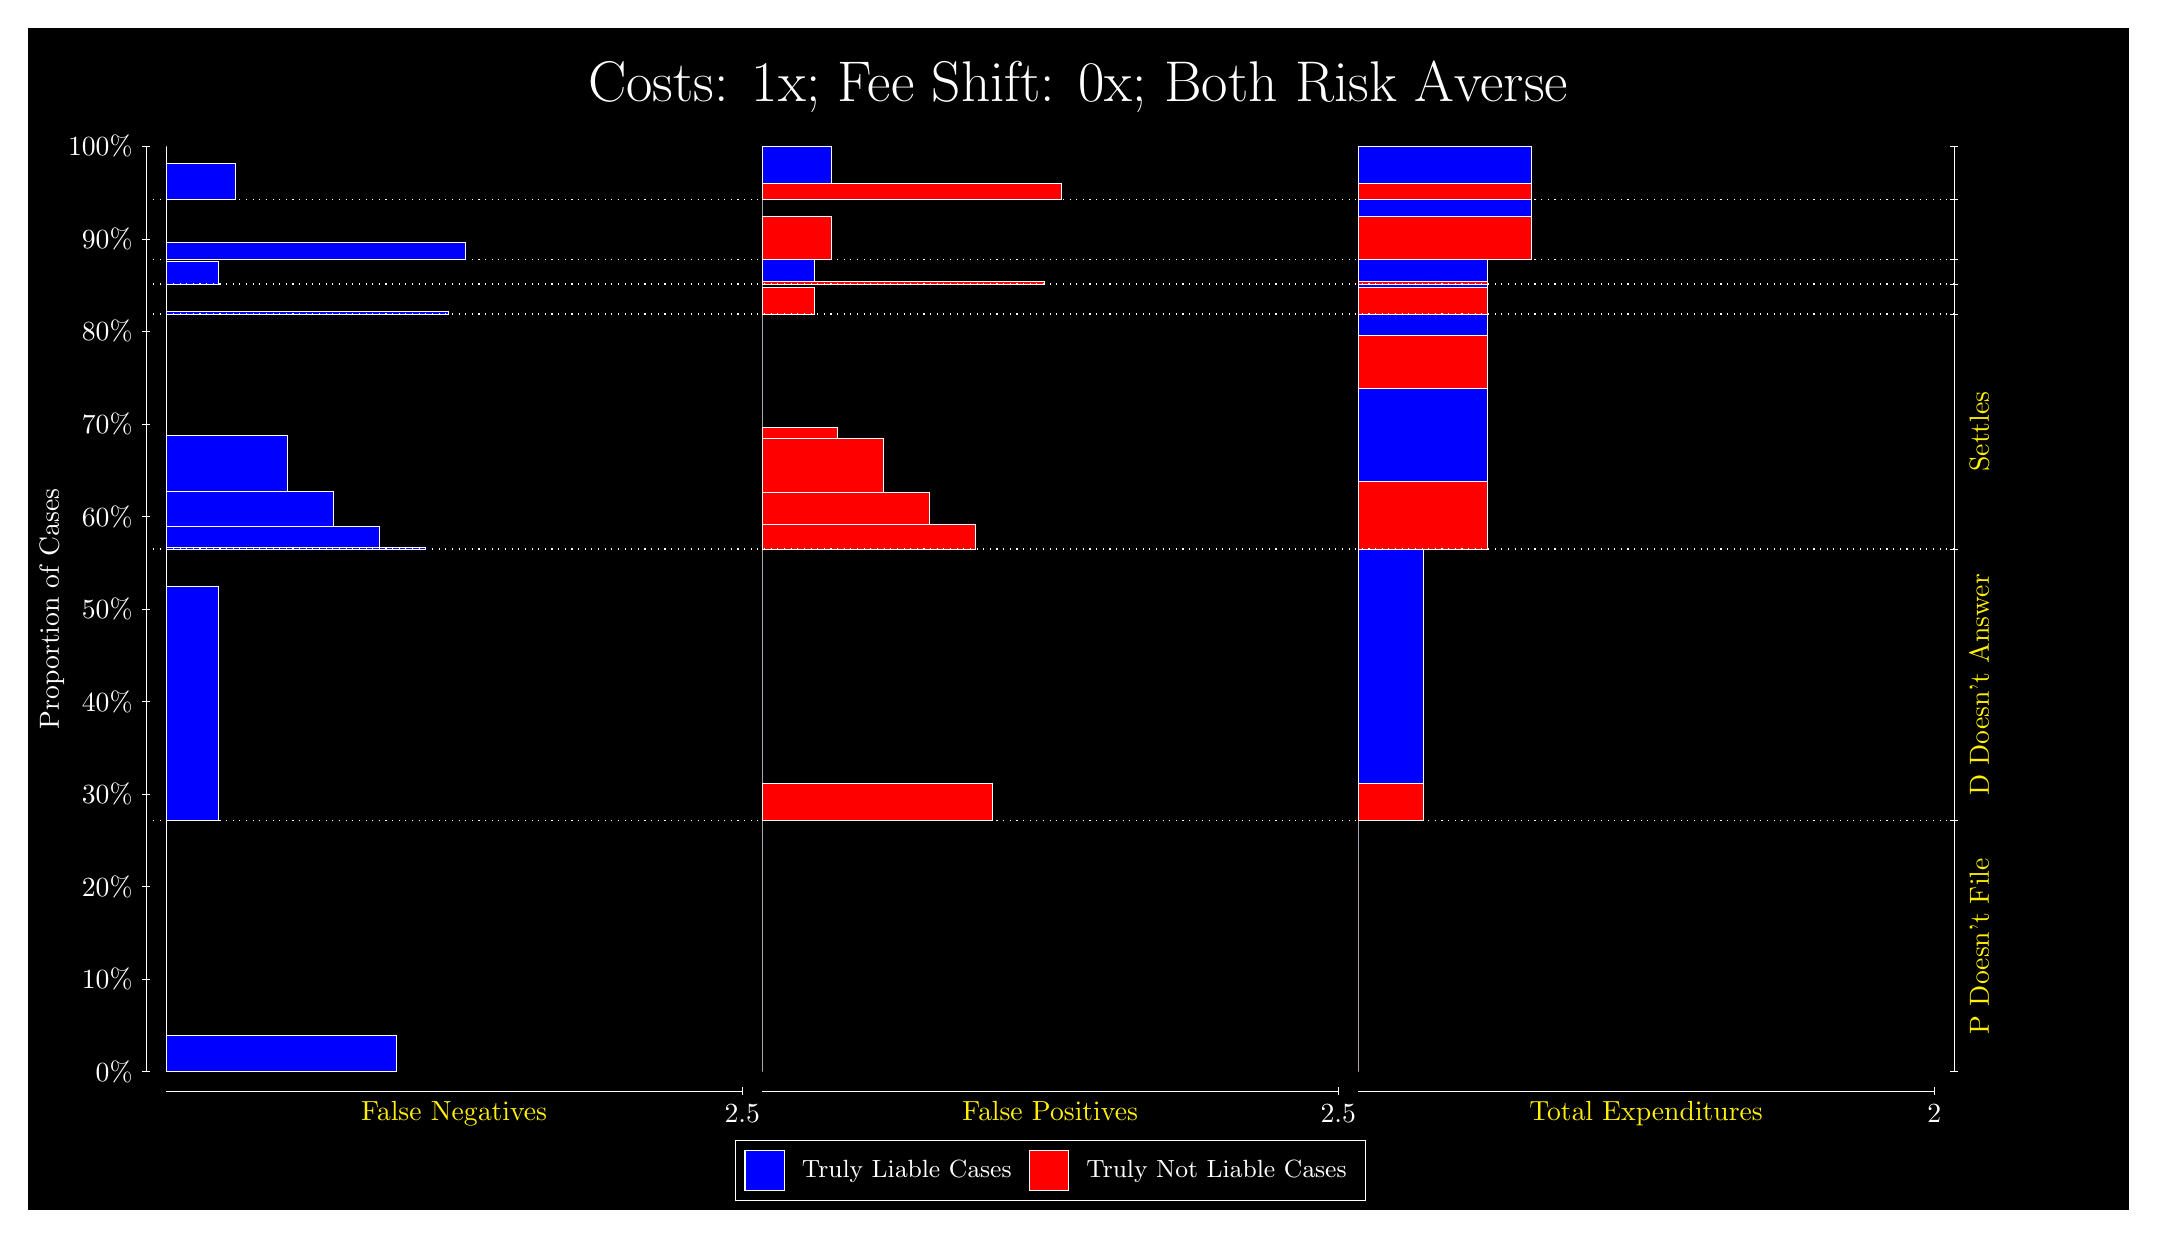
\begin{tikzpicture}
\draw[fill=black] (0,0) rectangle (26.667,15);
\draw[text=white] (0,13.5) rectangle (26.667,15) node[midway] {\huge Costs: 1x; Fee Shift: 0x; Both Risk Averse};
\draw[white, very thin] (1.5,1.75) -- (1.5,13.5);
\node[rotate=90, text=white, anchor=center] at (0.3, 7.625) {Proportion of Cases};
\draw[white, very thin] (1.45,1.75) -- (1.55,1.75);
\node[text=white, anchor=east] at (1.45, 1.75) {0\%};
\draw[white, very thin] (1.45,2.925) -- (1.55,2.925);
\node[text=white, anchor=east] at (1.45, 2.925) {10\%};
\draw[white, very thin] (1.45,4.1) -- (1.55,4.1);
\node[text=white, anchor=east] at (1.45, 4.1) {20\%};
\draw[white, very thin] (1.45,5.275) -- (1.55,5.275);
\node[text=white, anchor=east] at (1.45, 5.275) {30\%};
\draw[white, very thin] (1.45,6.45) -- (1.55,6.45);
\node[text=white, anchor=east] at (1.45, 6.45) {40\%};
\draw[white, very thin] (1.45,7.625) -- (1.55,7.625);
\node[text=white, anchor=east] at (1.45, 7.625) {50\%};
\draw[white, very thin] (1.45,8.8) -- (1.55,8.8);
\node[text=white, anchor=east] at (1.45, 8.8) {60\%};
\draw[white, very thin] (1.45,9.975) -- (1.55,9.975);
\node[text=white, anchor=east] at (1.45, 9.975) {70\%};
\draw[white, very thin] (1.45,11.15) -- (1.55,11.15);
\node[text=white, anchor=east] at (1.45, 11.15) {80\%};
\draw[white, very thin] (1.45,12.325) -- (1.55,12.325);
\node[text=white, anchor=east] at (1.45, 12.325) {90\%};
\draw[white, very thin] (1.45,13.5) -- (1.55,13.5);
\node[text=white, anchor=east] at (1.45, 13.5) {100\%};

\draw[white, very thin] (24.457,1.75) -- (24.457,13.5);
\draw[white, very thin] (24.407,1.75) -- (24.507,1.75);
\node[anchor=west] at (24.407, 1.75) {};
\draw[white, very thin] (24.407,4.9346) -- (24.507,4.9346);
\node[anchor=west] at (24.407, 4.9346) {};
\draw[white, very thin] (24.407,8.3854) -- (24.507,8.3854);
\node[anchor=west] at (24.407, 8.3854) {};
\draw[white, very thin] (24.407,11.371) -- (24.507,11.371);
\node[anchor=west] at (24.407, 11.371) {};
\draw[white, very thin] (24.407,11.751) -- (24.507,11.751);
\node[anchor=west] at (24.407, 11.751) {};
\draw[white, very thin] (24.407,12.068) -- (24.507,12.068);
\node[anchor=west] at (24.407, 12.068) {};
\draw[white, very thin] (24.407,12.826) -- (24.507,12.826);
\node[anchor=west] at (24.407, 12.826) {};
\draw[white, very thin] (24.407,13.5) -- (24.507,13.5);
\node[anchor=west] at (24.407, 13.5) {};

\draw[white, very thin, fill=blue] (1.75,1.75) rectangle (4.6775,2.2104);
\draw[white, very thin, fill=red] (1.75,2.2104) rectangle (1.75,4.9346);
\draw[white, very thin, fill=blue] (1.75,4.9346) rectangle (2.4087,7.912);
\draw[white, very thin, fill=red] (1.75,7.912) rectangle (1.75,8.3854);
\draw[white, very thin, fill=blue] (1.75,8.3854) rectangle (5.0435,8.4049);
\draw[white, very thin, fill=blue] (1.75,8.4049) rectangle (4.458,8.6726);
\draw[white, very thin, fill=blue] (1.75,8.6726) rectangle (3.8725,9.115);
\draw[white, very thin, fill=blue] (1.75,9.115) rectangle (3.287,9.8264);
\draw[white, very thin, fill=red] (1.75,9.8264) rectangle (1.75,11.371);
\draw[white, very thin, fill=blue] (1.75,11.371) rectangle (5.3362,11.41);
\draw[white, very thin, fill=red] (1.75,11.41) rectangle (1.75,11.751);
\draw[white, very thin, fill=blue] (1.75,11.751) rectangle (2.4087,12.035);
\draw[white, very thin, fill=red] (1.75,12.035) rectangle (1.75,12.068);
\draw[white, very thin, fill=blue] (1.75,12.068) rectangle (5.5558,12.278);
\draw[white, very thin, fill=red] (1.75,12.278) rectangle (1.75,12.826);
\draw[white, very thin, fill=blue] (1.75,12.826) rectangle (2.6283,13.291);
\draw[white, very thin, fill=red] (1.75,13.291) rectangle (1.75,13.5);
\draw[white, very thin, fill=red] (9.3189,1.75) rectangle (9.3189,4.4742);
\draw[white, very thin, fill=blue] (9.3189,4.4742) rectangle (9.3189,4.9346);
\draw[white, very thin, fill=red] (9.3189,4.9346) rectangle (12.246,5.4079);
\draw[white, very thin, fill=blue] (9.3189,5.4079) rectangle (9.3189,8.3854);
\draw[white, very thin, fill=red] (9.3189,8.3854) rectangle (12.027,8.6973);
\draw[white, very thin, fill=red] (9.3189,8.6973) rectangle (11.441,9.1091);
\draw[white, very thin, fill=red] (9.3189,9.1091) rectangle (10.856,9.7887);
\draw[white, very thin, fill=red] (9.3189,9.7887) rectangle (10.27,9.9301);
\draw[white, very thin, fill=blue] (9.3189,9.9301) rectangle (9.3189,11.371);
\draw[white, very thin, fill=red] (9.3189,11.371) rectangle (9.9776,11.713);
\draw[white, very thin, fill=blue] (9.3189,11.713) rectangle (9.3189,11.751);
\draw[white, very thin, fill=red] (9.3189,11.751) rectangle (12.905,11.784);
\draw[white, very thin, fill=blue] (9.3189,11.784) rectangle (9.9776,12.068);
\draw[white, very thin, fill=red] (9.3189,12.068) rectangle (10.197,12.617);
\draw[white, very thin, fill=blue] (9.3189,12.617) rectangle (9.3189,12.826);
\draw[white, very thin, fill=red] (9.3189,12.826) rectangle (13.125,13.036);
\draw[white, very thin, fill=blue] (9.3189,13.036) rectangle (10.197,13.5);
\draw[white, very thin, fill=red] (16.888,1.75) rectangle (16.888,4.4742);
\draw[white, very thin, fill=blue] (16.888,4.4742) rectangle (16.888,4.9346);
\draw[white, very thin, fill=red] (16.888,4.9346) rectangle (17.711,5.4079);
\draw[white, very thin, fill=blue] (16.888,5.4079) rectangle (17.711,8.3854);
\draw[white, very thin, fill=red] (16.888,8.3854) rectangle (18.534,9.2505);
\draw[white, very thin, fill=blue] (16.888,9.2505) rectangle (18.534,10.424);
\draw[white, very thin, fill=red] (16.888,10.424) rectangle (18.534,11.104);
\draw[white, very thin, fill=blue] (16.888,11.104) rectangle (18.534,11.371);
\draw[white, very thin, fill=red] (16.888,11.371) rectangle (18.534,11.713);
\draw[white, very thin, fill=blue] (16.888,11.713) rectangle (18.534,11.751);
\draw[white, very thin, fill=red] (16.888,11.751) rectangle (18.534,11.784);
\draw[white, very thin, fill=blue] (16.888,11.784) rectangle (18.534,12.068);
\draw[white, very thin, fill=red] (16.888,12.068) rectangle (19.083,12.617);
\draw[white, very thin, fill=blue] (16.888,12.617) rectangle (19.083,12.826);
\draw[white, very thin, fill=red] (16.888,12.826) rectangle (19.083,13.036);
\draw[white, very thin, fill=blue] (16.888,13.036) rectangle (19.083,13.5);
\draw[white, dotted] (1.5,4.9346) -- (24.457,4.9346);
\draw[white, dotted] (1.5,8.3854) -- (24.457,8.3854);
\draw[white, dotted] (1.5,11.371) -- (24.457,11.371);
\draw[white, dotted] (1.5,11.751) -- (24.457,11.751);
\draw[white, dotted] (1.5,12.068) -- (24.457,12.068);
\draw[white, dotted] (1.5,12.826) -- (24.457,12.826);
\draw[white, very thin] (1.75,1.5) -- (9.0689,1.5);
\node[text=yellow, anchor=north] at (5.4094, 1.5) {False Negatives};
\draw[white, very thin] (9.0689,1.45) -- (9.0689,1.55);
\node[text=white, anchor=north] at (9.0689, 1.45) {2.5};

\draw[white, very thin] (9.3189,1.5) -- (16.638,1.5);
\node[text=yellow, anchor=north] at (12.978, 1.5) {False Positives};
\draw[white, very thin] (16.638,1.45) -- (16.638,1.55);
\node[text=white, anchor=north] at (16.638, 1.45) {2.5};

\draw[white, very thin] (16.888,1.5) -- (24.207,1.5);
\node[text=yellow, anchor=north] at (20.547, 1.5) {Total Expenditures};
\draw[white, very thin] (24.207,1.45) -- (24.207,1.55);
\node[text=white, anchor=north] at (24.207, 1.45) {2};

\node[text=yellow, centered, rotate=90] at (24.777, 3.3423) {P Doesn't File};
\node[text=yellow, centered, rotate=90] at (24.777, 6.66) {D Doesn't Answer};
\node[text=yellow, centered, rotate=90] at (24.777, 9.8783) {Settles};





\draw (12.978300999999998,1.5) node[draw=none] (baseCoordinate) {};
\begin{scope}[align=center]
        \matrix[scale=0.5, draw=white, below=0.5cm of baseCoordinate, nodes={draw}, column sep=0.1cm]{
            \node[rectangle, draw, minimum width=0.5cm, minimum height=0.5cm, fill=blue] {}; &
            \node[draw=none, font=\small, text=white] (B) {Truly Liable Cases}; &
            \node[rectangle, draw, minimum width=0.5cm, minimum height=0.5cm, fill=red] {}; &
            \node[draw=none, font=\small, text=white] (B) {Truly Not Liable Cases}; \\
            };
\end{scope}

\end{tikzpicture}
\end{document}